\chapter{Proposta Conceitual}

Esta seção apresenta uma proposta de utilização de \textit{templates} multicamadas para criar e manipular questões de programação. A ideia inclui o emprego de inteligência artificial generativa como ferramenta complementar, responsável por sugerir variações criativas no \textit{template} base, tais como modificações de contexto, acréscimo de novos cenários e introdução de pontos de variação. Além disso, a IA generativa também oferece suporte no fornecimento de \textit{feedback} imediato ao estudante após a submissão da resposta, apontando erros, sugerindo melhorias e apresentando explicações detalhadas sobre o problema e possíveis soluções. 

\section{Geral para o Específico}
A geração automática de questões segue um processo hierárquico que se inicia em tópicos mais amplos e evolui até questões específicas. Em primeiro lugar, são definidos os tópicos da ementa, que correspondem a áreas ou domínios do conhecimento a serem avaliados (por exemplo, Estruturas de Repetição, Estruturas de Decisão, Matrizes, Funções). Esses tópicos abrangem conteúdos específicos do currículo e orientam a elaboração dos modelos cognitivos. Na etapa seguinte, estes modelos cognitivos são convertidos em \textit{templates}, que servirão de base para a geração das questões. Essa abordagem reflete a metodologia recomendada para a criação de questões baseadas em \textit{templates}. 

\begin{figure}[ht]
	\centering
	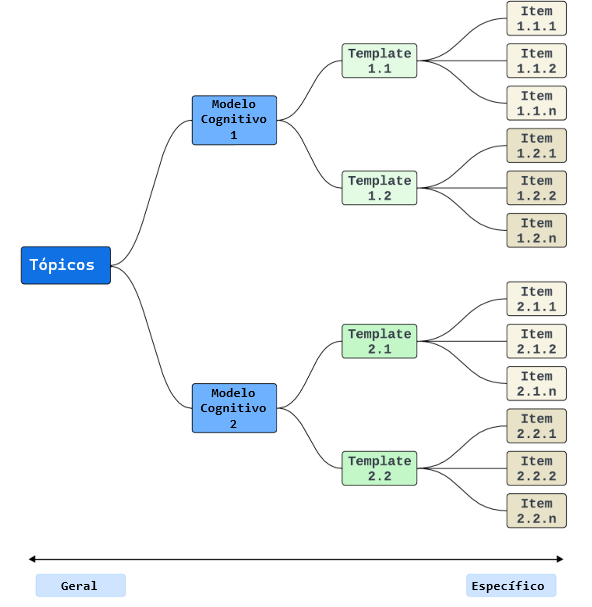
\includegraphics[width=14cm]{./imagens/capitulo5/geral-especifico-com-topicos}
	\caption{Geral para o específico, (adaptado, \cite{hendrickson2010}) }
	\label{fig:geral-to-specif}
\end{figure}


\section{Escala de proficiência}

A classificação das questões com base em atributos e características, como o nível de dificuldade, é essencial nas avaliações educacionais. Agrupar questões por níveis de dificuldade (fácil, médio e difícil) possibilita organizar bancos de questões que atendem diferentes perfis de estudantes.  Esse agrupamento é especialmente relevante em contextos que utilizam testes adaptativos , onde o sistema ajusta a dificuldade das questões apresentadas de acordo com o nível de aptidão do aluno. Assim, é possível proporcionar uma experiência de aprendizado personalizada, onde cada questão apresentada se adequa ao desempenho e à evolução do aluno ao longo das avaliações. \textbackslash{}\parencite{pasquali2018}. 


A figura \ref{fig:proficiency-scale}  ilustra um banco de modelos estruturado para oferecer templates compatíveis com diferentes níveis de dificuldade. Esse tipo de organização permite um maior controle sobre a dificuldade das questões geradas.


\begin{figure}[ht]
	\centering
	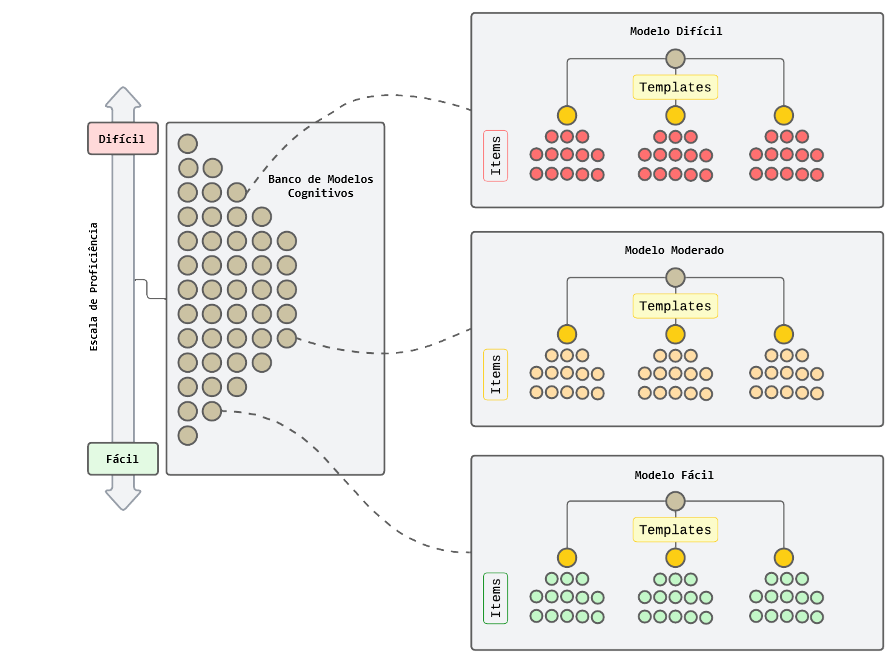
\includegraphics[width=14cm]{./imagens/capitulo5/proficiency-scale-named}
	\caption{Geral para o específico, (adaptado, \cite{hendrickson2010}) }
	\label{fig:proficiency-scale}
\end{figure}

\section{Estrutura dos Templates em JSON}

O JSON foi adotado como formato padrão para a construção dos templates de questões devido ao seu alto desempenho, simplicidade e facilidade de uso. Em comparação ao XML, o JSON mostrou-se mais eficiente em diversas métricas, conforme demonstrado no trabalho de \parencite{wang2011}, que indica um ganho de  48,56\% na velocidade de carregamento de 1000 objetos por página comparado com o XML. Esse resultado deve-se, em grande parte, à estrutura mais enxuta do JSON, que demanda menos esforço de interpretação se comparado ao uso extensivo de \textit{tags} no XML.  Além disso, o JSON oferece suporte nativo a tipos de dados como \textit{arrays}, números, \textit{strings} e valores booleanos, o que simplifica o tratamento de estruturas hierárquicas — característica fundamental na representação de templates de questões.

\begin{figure}[ht]
	\centering
	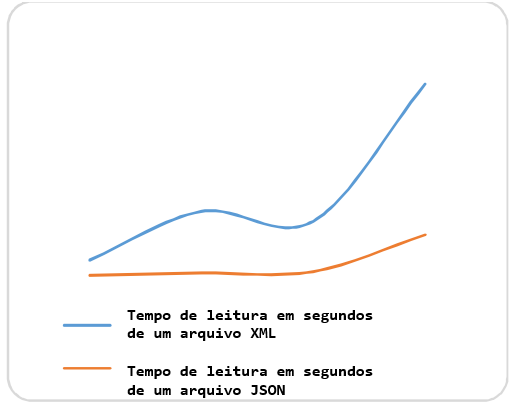
\includegraphics[width=10cm]{./imagens/capitulo5/json-vs-xml}
	\caption{comparação de leitura JSON vs XML, \parencite{goyal2017} }
	\label{fig:json-vs-xml}
\end{figure}

Outro fator relevante é a compatibilidade do JSON com linguagens modernas, como JavaScript, Python e Java, eliminando a necessidade de bibliotecas externas para análise (\textit{parsing}) ou manipulação de dados. Já o XML frequentemente exige mais recursos para tratamento de \textit{tags} e maior esforço de processamento. A análise de desempenho citado por \parencite{goyal2017} destaca que o JSON, por ser mais leve e simples, tem melhor tempo de leitura em aplicações com pares de chave-valor, conforme a figura \ref{fig:json-vs-xml}. Assim, sua adoção torna o desenvolvimento de sistemas mais eficiente e escalável, justificando sua escolha como formato preferencial para os templates de questões neste trabalho.


\section{Representação Hierárquica dos Templates em JSON}

Inicialmente, escrever o modelo de questão em um editor de texto é uma prática útil para planejar a estrutura do template. No entanto, a fase seguinte envolve a estruturação desse modelo em formato JSON, o que facilita a manipulação e a geração de questões de forma automatizada. A transição para JSON permite que o template seja facilmente editado e gerenciado, permitindo o desenvolvimento de \textit{scripts} ou algoritmos capazes de gerar automaticamente diversas instâncias de questões a partir do template.
A Figura \ref{fig:template-json-example-1} ilustra como o template pode ser organizado no formato JSON, composto por três componentes principais: Texto Principal (\textit{Stem}), Variáveis e as Multicamadas (\textit{N-Layers}). Cada elemento desempenha um papel específico conforme as seguintes finalidades:


\begin{itemize} \item \textbf{Texto Principal (\textit{Stem})} \begin{itemize} \item Representa o texto base da questão, servindo de ponto de partida para a formulação do template. Nele contém trechos fixos e indicações de onde as variáveis serão inseridas, tornando a questão adaptável a diferentes contextos. \end{itemize}
\item \textbf{Variáveis (\textit{Variables})}
\begin{itemize}
    \item Inclui parâmetros e conteúdos que podem variar, permitindo a personalização do texto principal com indicações de onde serão inseridas no enunciado, de forma que permita a flexibilidade e reutilização destas variáveis em outros cenários.
\end{itemize}

\item \textbf{Multicamadas (\textit{N-Layers})}
\begin{itemize}
    \item Funcionam como \textit{subtemplates} dentro do template principal, que possibilita a inclusão de novas variáveis e conteúdos para expandir e adaptar o enunciado da questão em diferentes cenários, um sub-layer sempre deriva do template principal.
    \end{itemize}
\end{itemize}


\begin{figure}[ht]
	\centering
	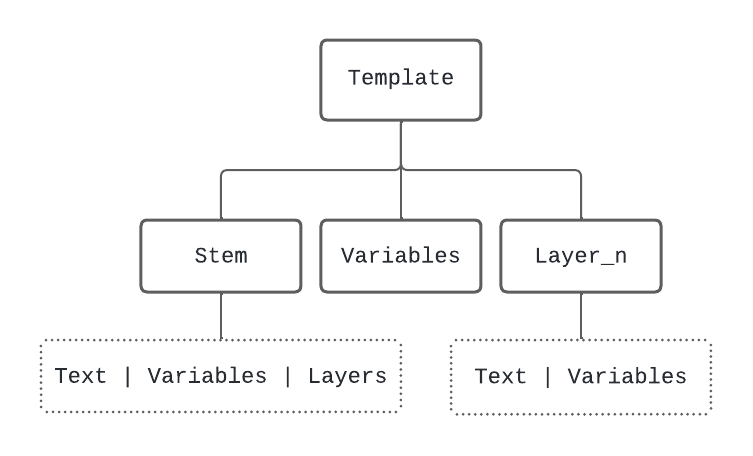
\includegraphics[width=14cm]{./imagens/capitulo5/template-json-example-1}
	\caption{Estrutura do template de questões (Elaboração Própria, 2025) }
	\label{fig:template-json-example-1}
\end{figure}


\section{Mecanismo de Combinação}

O mecanismo de combinação consiste em um processo de geração de questões a partir do \textit{template} principal, descrito no formato JSON, que contém estruturas de texto e múltiplas opções de conteúdo. Esse \textit{template} atua como um conjunto de possibilidades, permitindo que novas perguntas sejam criadas de forma sistemática, por meio da seleção e combinação das variações de cada campo.

Para que o \textit{template} seja aplicado em diferentes cenários, é utilizado um segundo arquivo JSON onde cada chave representa a configuração de uma questão específica e cada valor corresponde ao índice selecionado em cada campo do \textit{template}. Dessa forma, se no campo \textbf{"introduction": ["intro\_1", intro\_2", "intro\_3"]} se a questão exigir a segunda opção, o valor referenciado será o índice \texttt{\textbf{1}} (assumindo zero como base de indexação). Essa abordagem sistematiza a produção automatizada de questões, pois basta apenas alterar os índices para gerar combinações distintas, sem alterar a estrutura original do texto.

A Figura \ref{fig:template-1} (referente ao \textit{template}) e a Figura \ref{fig:template-2} (referente às instâncias de questões) ilustram esse processo. Enquanto a primeira foca nos template em si e seus valores possíveis, a segunda demonstra como cada questão seleciona um conjunto de índices para formar a questão final. 

\begin{figure}[ht]
	\centering
	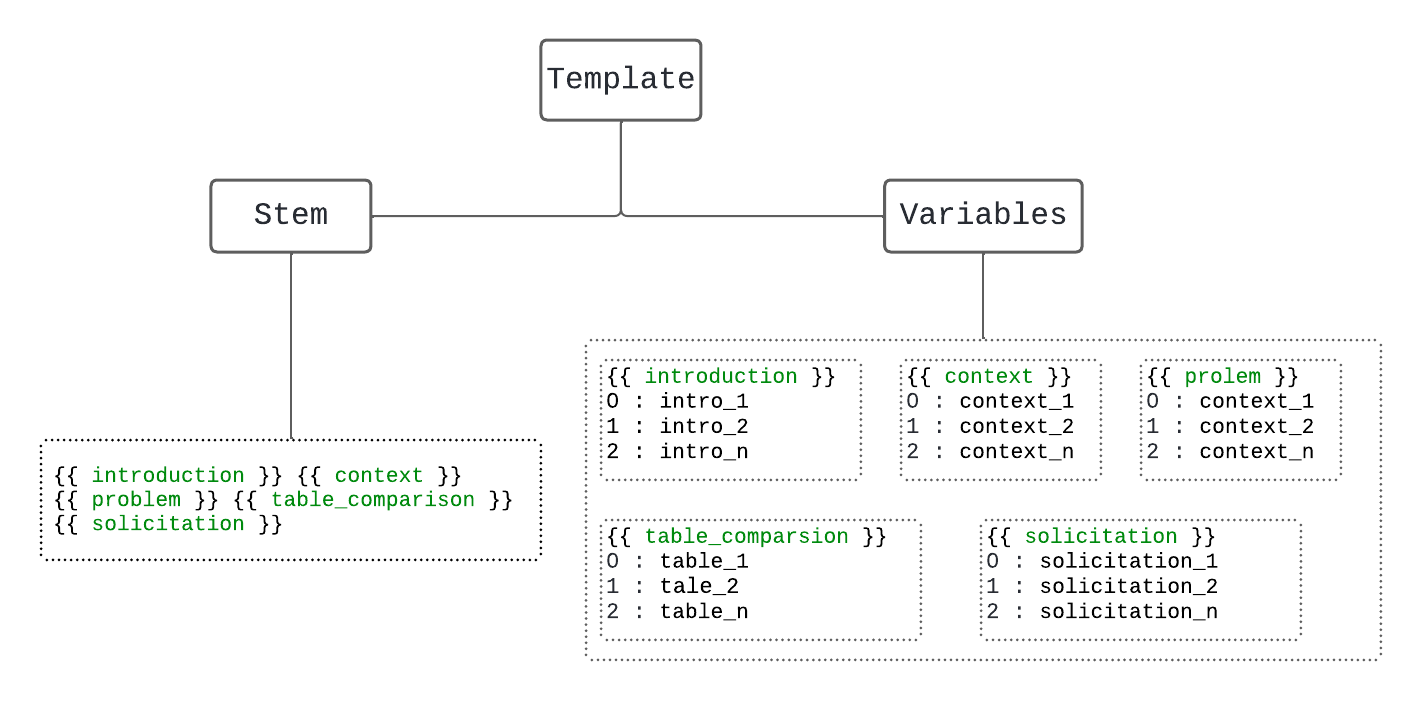
\includegraphics[width=16cm]{./imagens/capitulo5/template-1}
	\caption{JSON : Template Principal (Elaboração Própria, 2025) }
	\label{fig:template-1}
\end{figure}

\begin{figure}[ht]
	\centering
	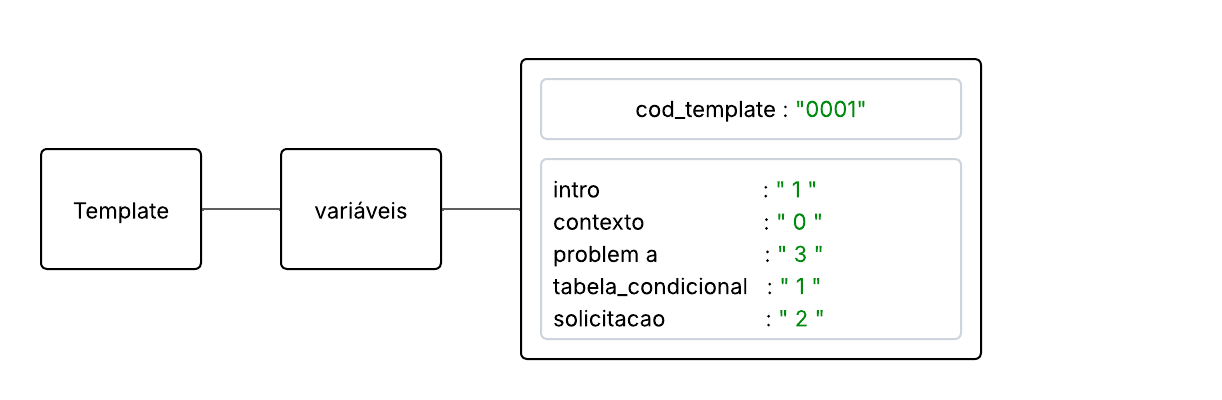
\includegraphics[width=14cm]{./imagens/capitulo5/template-2}
	\caption{Template de Questões (Elaboração Própria, 2025) }
	\label{fig:template-2}
\end{figure}

\section{Algoritmos Utilizados}

Nesta seção será apresentado os algoritmos empregados para gerar as questões de forma automática a partir de dois arquivos JSON distintos: um contendo o template (JSON de Template), e outro contendo as questões (JSON de Questão). O \textit{JSON de Template} reúne a estrutura de cada parte de uma questão e as possíveis variações de conteúdo que podem ser combinadas. Já o \textit{JSON de Questões} consiste em um conjunto de chaves que apontam para índices específicos dentro das listas de opções do \textit{JSON Template}, permitindo a criação de múltiplas versões a partir de um único template. 
Para construção das questões, foram definidas duas funções principais conforme o cabeçalho de código \ref{cod:cabecalho}, a primeira função é responsável por percorrer os índices litados no JSON de Questões e, a partir disso, combinar cada elemento com os respectivo campo do JSON de Template, retornando todas as questões geradas. A segunda função retorna uma única questão específica, desde que seja fornecido o código (ou índice) correspondente para delimitar o tipo de busca por questões específicas.


\begin{listing}[ht]
\begin{minted}[linenos=true, autogobble, bgcolor=Cornsilk1]{c}
# cabeçalho da função 1
generate_all_questions(json_template, json_questions)

# cabeçalho da funcao 2
generate_one_question(json_template, json_questions, id=None) 
\end{minted}
\caption{cabeçalho das funções de geração de questões (Autoria Propria, 2025)}
\label{cod:cabecalho}
\end{listing}

    
\section{Fluxo de Trabalho}

O fluxo de trabalho descrito no \gls{bpmn} na figura \ref{fig:bpmn-fluxo} organiza de forma colaborativa as interações entre professor (especialista), inteligência artificial (IA) e aluno no contexto de geração automática de questões. Esse fluxo de trabalho tem como objetivo auxliar a criação e validação das questões, bem como o fornecimento de \textit{beedback} para os estudantes. 

O \textbf{professor} (especialista) define define os modelos cognitivos  e elabora os templates de questões. Em seguida, o professor realiza a validação dos pontos de variação dos \textit{templates}, garantindo que as questões propostas pela IA estejam alinhadas aos objetivos pedagógicos.

No papel da IA, há duas etapas principais: primeiramente, a IA é responsável por propor variações das questões a partir dos \textit{templates}, criando cenários  que atendam a diferentes contextos e perfis de aprendizagem. Posteriormente, a IA analisa as respostas enviadas pelos alunos, identificando possíveis erros ou inconsistências. Com base nessa análise, a IA sugere correções e melhorias que podem ser implementadas nos códigos ou nos argumentos apresentados.

E por fim, o aluno é o principal beneficiário desse processo. Ele recebe as questões geradas, responde por meio do sistema e obtém feedback em tempo real. Esse retorno rápido permite que o aluno ajuste sua compreensão sobre o assunto estudado. 

\begin{figure}[ht]
	\centering
	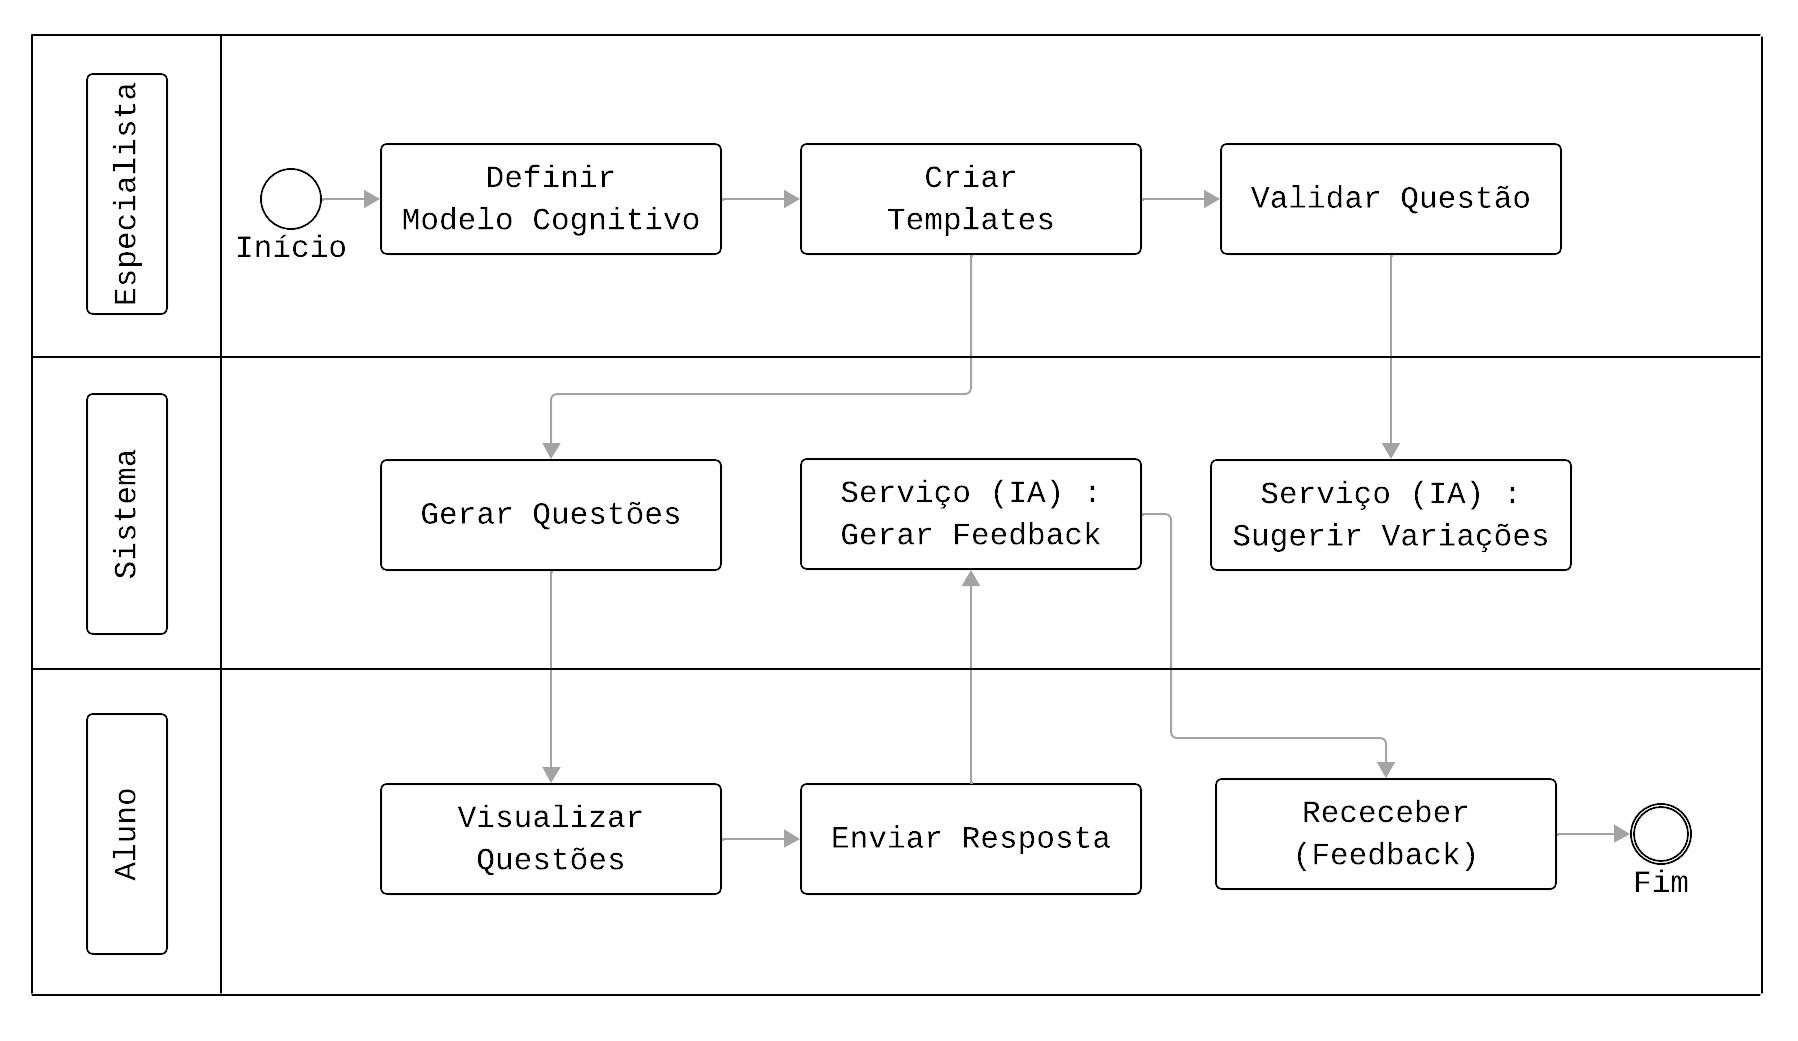
\includegraphics[width=16cm]{./imagens/capitulo6/bpmn-fluxo}
	\caption{BPMN do Fluxo de Trabalho (Elaboração Própria, 2025) }
	\label{fig:bpmn-fluxo}
\end{figure}